\documentclass[letterpaper,11pt]{article}

\usepackage{graphicx}
\usepackage{multicol}
\usepackage{fullpage}
\usepackage{csquotes}
\usepackage[margin=0.75in,letterpaper]{geometry}
\setlength{\footskip}{15pt}
\setlength{\belowcaptionskip}{9pt}
\usepackage{censor}
\usepackage{floatflt}
\usepackage{xspace}
\usepackage[margin=1cm,skip=9pt]{caption}
\usepackage{ulem}
\usepackage{tikz}
\usetikzlibrary{shadows}

% https://tex.stackexchange.com/questions/5226/keyboard-font-for-latex
\newcommand*\keys[1]{%
  \tikz[baseline=(key.base)]
    \node[%
      draw,
      fill=white,
      drop shadow={shadow xshift=0.25ex,shadow yshift=-0.25ex,fill=black,opacity=0.75},
      rectangle,
      rounded corners=2pt,
      inner sep=1pt,
      line width=0.5pt,
      minimum width=1.1em,
      font=\scriptsize\sffamily
    ](key) {#1\strut}
  ;
}

\linespread{0.95}
\def\degC{$^{\circ}$C }
\def\degf{$^{\circ}$F }
\def\vol #1 {{\bf #1}, $\;\;$}
\def\refer{\par\noindent\hangindent\parindent\hangafter1}


\title{\vspace{-2.0cm}Herzmann Family Christmas Letter 2022}
\author{Daryl Herzmann${}^1$, Elizabeth Herzmann${}^2$, Margaret 
Herzmann${}^3$,\\
Robert Herzmann${}^4$, AND Charlotte Herzmann${}^4$ \\
\textit{${}^1$Proprietor},
\it{${}^2$Responsible Adult},
\it{${}^3$Almost Ten},
\it{${}^4$Additional Children}}
\date{13 December 2022}

\makeatletter
\newenvironment{tablehere}
  {\def\@captype{table}}
  {}

\newenvironment{figurehere}
  {\def\@captype{figure}}
  {}
\makeatother

\newcommand{\Line}[0]{%
  \rule{0cm}{0cm}\\\hrule\rule{0cm}{0cm}%
}

%\addtolength{\textheight}{1.5in}

\begin{document}
\maketitle
\vspace{-0.75cm}
\begin{abstract}
Now is a propitious time and setting for an unabridged accounting of our
family's activities per annum.  The experienced reader should have already
prepared fully for what is to follow.
\end{abstract}

\vspace{-0.5cm}

\noindent\makebox[\linewidth]{\rule{\textwidth}{1pt}}

\begin{multicols}{2}

\section{Materials and Methods} 

Our family now comprises Daryl
\enquote{Daryl} (44), Elizabeth \enquote{Liz} ($<$40),
Margaret \enquote{Maggie Moo} (9), Robert \enquote{Bob-bert} (8), and
Charlotte \enquote{Burger} (5). Our cat Snoopy forcibly crossed the Rainbow
Bridge at the age of 14 after a bout with cancer.  A private burial service
was held in our backyard, followed a few weeks later by a kind fox's
exhumation for the kids to say goodbye one last time.

\subsection{Housing and Domestics}

Our dwelling place remains unchanged for the past decade and continues the
vindictive promise Daryl made to the Realtor that we would never move, even after she
insisted that we would want to move after seven years.  The following equation
succinctly describes the contents of our house:

\[ \frac{d(\mathrm{stuff} + \mathrm{junk})}{dt} > 0 \]

The only construction project of note was backyard excavation to install some
drainage water management.  The kids are shown working in Figure 1 with no
known child labor laws violated in the process.  The infiltration was only
marginally improved, so the kids will have more digging work to do.

\bigskip

\begin{figurehere}
    \centering   
    \resizebox{.95\columnwidth}{!}{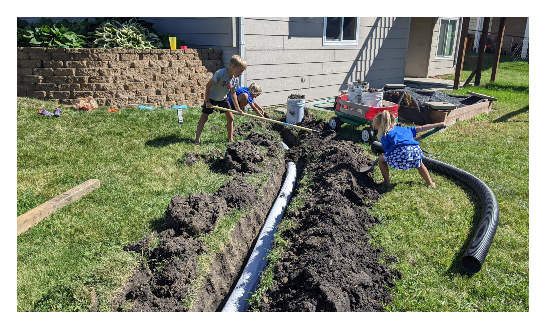
\includegraphics[angle=0]{plots/2022_f1.eps}}
    \caption{Children enjoying the pleasures of forced manual labor.}
\end{figurehere}

\subsection{Conveyances}

Herzmann et al. (2021) solicited donations for Liz's Ford F150 Lightning truck fund.
We generously received $8e^{-3}\%$ of the goal so far, thank you!  Liz's mini-van
experienced a break-in by nefarious actor(s), who made off with a paltry sum of
\$2 and many expired coupons.

\bigskip

\subsection{Employment}

Daryl remains gainfully employed by Iowa State University.  His primary work
tasks include soil erosion modeling and maintaining computer servers
running FORTRAN code, both circa the 20th century.

Liz still teaches at Southview Middle School here in Ankeny and keeps plenty busy with
church activities.  Note that the kids are in the "north side" system for Ankeny,
so as the name implies, their paths will not cross at school.  The highlight of
her year and for the first time in her teaching career, Liz broke up a fist
fight at school and lived to tell the tale.

The children don't seem interested in earning money for chores.
Instead they believe they are employed to bicker at each other, which perhaps if
we threatened to pay them for that work, they would then refuse to do it!

\section{Miss Charlotte}

Charlotte started kindergarten this fall and has been a very happy student.  She
has greatly benefited from watching and learning along side her kin. She contributes
the following text: "I love unicorns, I play outside, I like my dada, I love my mom."

Charlotte turns six in a few days and is very excited.  We'll denote her height
on the kitchen wall and then bemoan her lack of progress against her siblings.
She continues to underperform with stature, but Figure 2 should give her hope with an extrapolated
height of 222 $cm$ ($7'3"$) at age 18 and taller than both siblings.

\begin{figurehere}
    \centering   
    \resizebox{.95\columnwidth}{!}{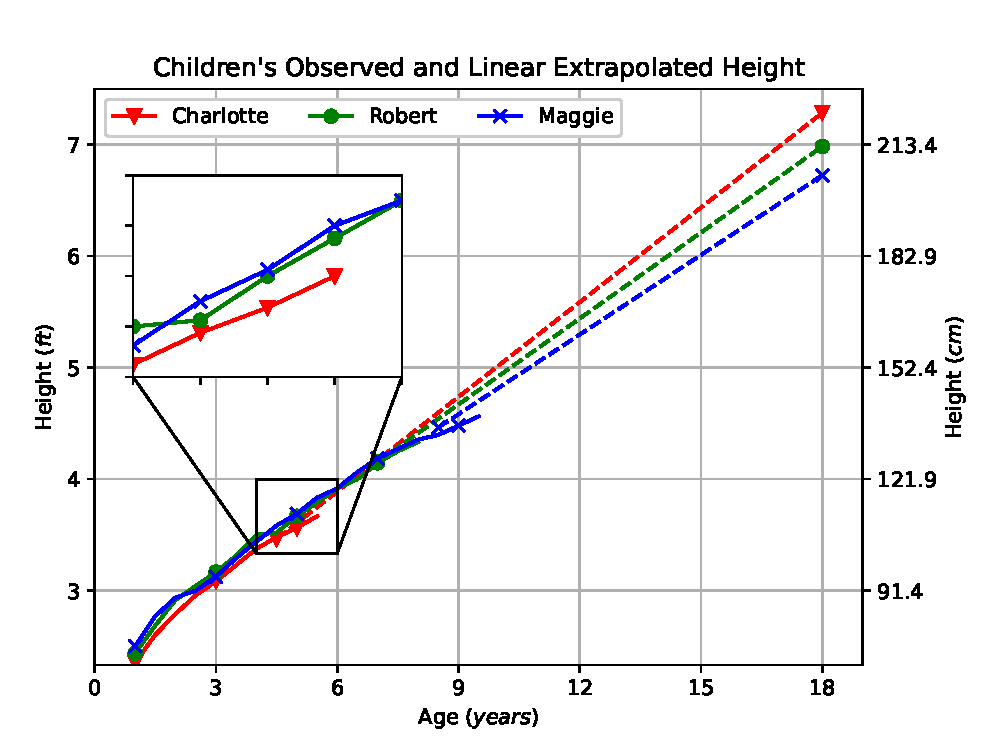
\includegraphics[angle=0]{plots/2022_f2.eps}}
    \caption{Observed and linear fit extrapolated height to the age of 18. Inset
    axis focuses year four to six observations.}
\end{figurehere}


\section{Mr Robert}

Robert writes: "I have many friends.
I am liking ${3}^{rd}$ grade. I have passed 10s in multiplication.
I got \textit{Minecraft} this year."  To expand on his terseness, he has been improving his
socialization skills, continues to excel at math, and enjoys playing video games.
He earned some money to purchase a computer game called "Farming Simulator 22"
and enjoys driving large combines on highways to disrupt local traffic.

We are proud that he continued to take piano lessons this fall and recently did
an excellent job at his recital.  He continues to see a positive benefit of learning
the piano for his academic work and penmanship. 

\section{Miss Maggie}

Maggie contributes "I'm in the ${4}^{th}$ grade and I love the subjects reading,
science and social studies. I have started alter serving at church (Figure 3) and
have loved to do it and always want to do more serving. Some activities I do are
dance, volleyball, and yearbook club at school. In yearbook club, we make the
school wide yearbooks." [\textit{editorial: aptly named club then...}]

She will be performing in the school wide talent show with her friends and will
have another dance recital in the spring.  She has a very kind heart and again
will be taking food pantry donations in lieu of gifts for her big 1-0 birthday
party in January.

\begin{figurehere}
    \centering   
    \resizebox{.95\columnwidth}{!}{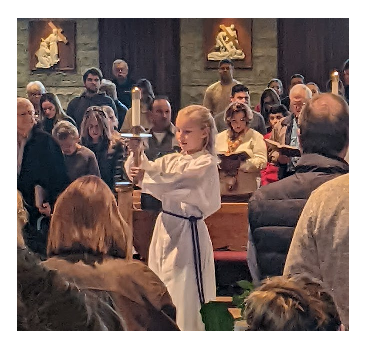
\includegraphics[angle=0]{plots/2022_f3.eps}}
    \caption{Maggie's first time alter serving. This painting was commissioned
    as we do not bring cellphones to church!}
\end{figurehere}

\section{Family Trips}

We went camping for the first time with Daryl's brother's family near Decorah.
We braved the outdoors within a modest log cabin with a modest air conditioner
and modest refrigerator.  The nearest indoor plumbing was about 200 meters away,
so survival was not assured.  The kids thoroughly enjoyed catching the same fish over
and over again.

Our family vacation trip was to the Rapid City area to see the standard sights:
Mount Rushmore, Badlands, and Wall Drug.  We planned it just before Sturgis, so
it was neat to see all the motorcycles and riff-raff in the area.  The kids were
most happy with mom's diligence to select hotels with the best pools along the
way.  Robert insisted on climbing every big rock encountered with Charlotte
following after him.

\bigskip

\emph{Acknowledgments} Our family wishes to thank you for the generous 
support, prayers, cards, gifts, and visits you have provided us in the past
year. A pay increase for Daryl covered color page charges for this diatribe.  Full
\LaTeX\xspace source of this letter can be found on Daryl's Github page. 

\section{References}

\refer Github, 2022: https://github.com/akrherz/akrherz , visited 13 Dec 2022.
\refer Herzmann, Daryl E., et al. Herzmann Family Christmas Letter, 2021.

\end{multicols}

\end{document}
